\documentclass[tikz,border=10pt]{standalone}
\usepackage[T1]{fontenc}
\usepackage{helvet}
\renewcommand{\familydefault}{\sfdefault}

\begin{document}
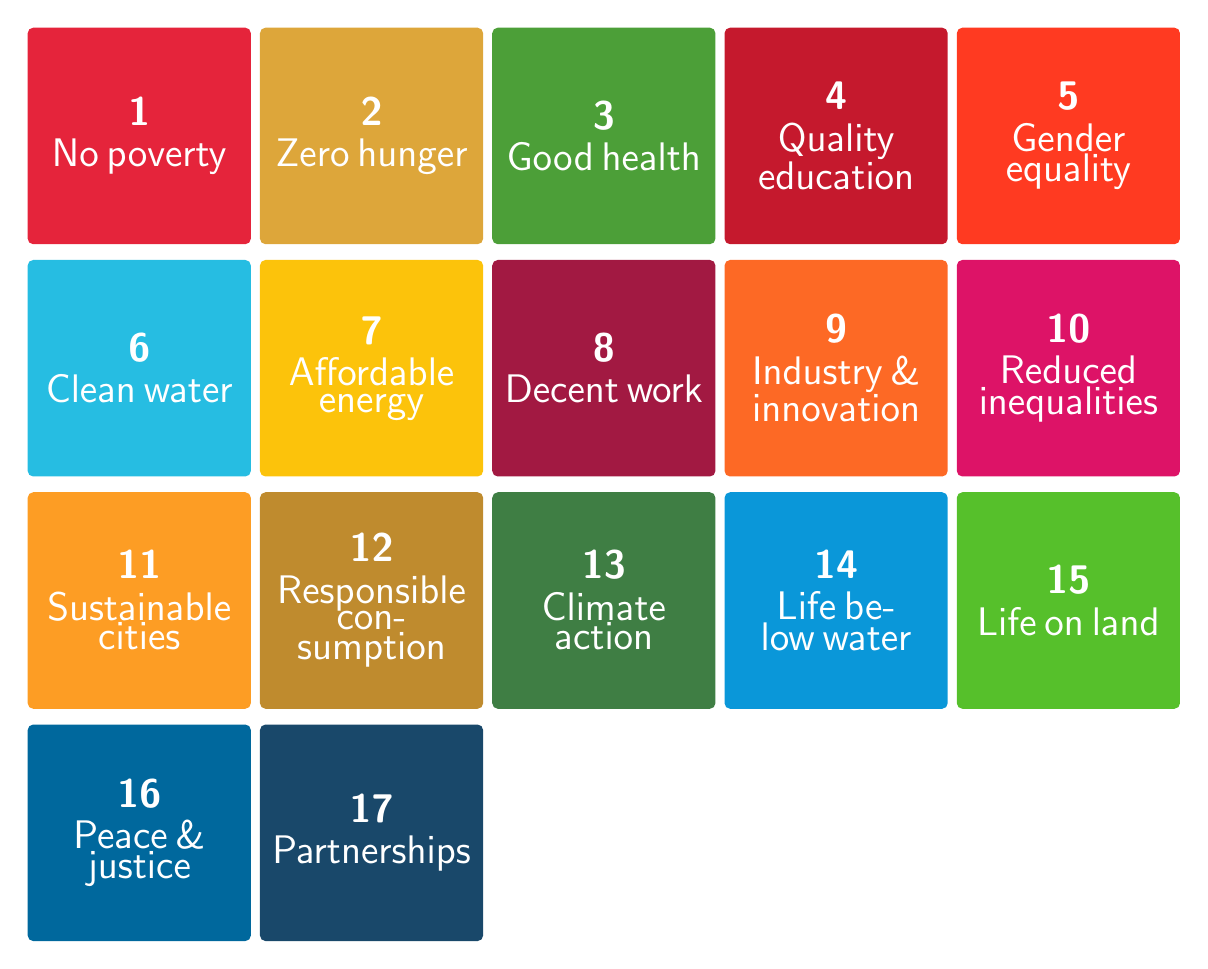
\begin{tikzpicture}[
  goal/.style={rounded corners=2pt, minimum width=2.75cm, minimum height=2.75cm,
               text width=2.6cm, align=center, text=white, font=\footnotesize},
  x=2.95cm, y=2.95cm
]

  % Liste: Spalte/Zeile/HTML-Farbe/Nummer/Kurztitel
  \foreach [count=\n from 0] \hex/\num/\title in {
    E5243B/1/No poverty,
    DDA63A/2/Zero hunger,
    4C9F38/3/Good health,
    C5192D/4/Quality education,
    FF3A21/5/Gender equality,
    26BDE2/6/Clean water,
    FCC30B/7/Affordable energy,
    A21942/8/Decent work,
    FD6925/9/Industry \& innovation,
    DD1367/10/Reduced inequalities,
    FD9D24/11/Sustainable cities,
    BF8B2E/12/Responsible consumption,
    3F7E44/13/Climate action,
    0A97D9/14/Life below water,
    56C02B/15/Life on land,
    00689D/16/Peace \& justice,
    19486A/17/Partnerships
  }{
    \definecolor{tmpcolor}{HTML}{\hex}
    \pgfmathsetmacro{\x}{mod(\n,5)}
    \pgfmathsetmacro{\y}{-floor(\n/5)}
    \node[goal, fill=tmpcolor] at (\x,\y) {\Large\textbf{\num}\\[4pt]\title};
  }

\end{tikzpicture}
\end{document}